\documentclass[10.5pt, a4j, twocolumn]{jsarticle}


\usepackage[dvipdfm,margin=1.5cm]{geometry}% 余白の調整 上下左右 = 2 cm
\usepackage[dvipdfmx]{graphicx, color}% 画像の読み込み
\usepackage{type1cm}% おまじない
\usepackage{url}% URL の記述のため
\usepackage{fancybox,ascmac}
\usepackage{fancyhdr} %ヘッダーを入れるため
\usepackage{txfonts}
\usepackage{cite}
\setlength\intextsep{2pt}
\setlength\textfloatsep{2pt}


\renewcommand{\baselinestretch}{1}

%citeの括弧を全角にするおまじない
\renewcommand{\citeleft}{\inhibitglue{}[}
\renewcommand{\citeright}{]{}\inhibitglue}
\makeatletter
 \renewcommand\@biblabel[1]{\inhibitglue{}[#1]{}\inhibitglue}
\makeatother


\setlength{\abovecaptionskip}{0mm}
\setlength{\belowcaptionskip}{0mm}


\begin{document}

\title{マルチエージェントシミュレーションによる不規則動詞の規則化に対する人口流入の影響\\       }

\date{}
\author{東条研究室 \\ 1310034 鈴木啓章}

\maketitle % 表題
\thispagestyle{fancy}
 \lhead{2014年9月1日 中間審査}
%\vspace{-20mm}


\section{はじめに}\label{sec:intro}
現在の日常的に用いられている不規則動詞はおおよそ180語存在し、
会話の中に出現する動詞の約70\%が
不規則動詞である(be, have,etc...)\cite{pinker}.これらの不規則動詞はOld English時代[AD 800 頃]に強変化動詞(strong verb)と呼ばれ主に母音が変化することによって現在形、過去形、過去分詞などの活用形が生成されていた.
Modern Englishでは例外も含め9クラスに分類され、クラス内にも細かい分類がなされている\cite{pinker2}.
しかし、上記の不規則動詞には単純に接尾辞[-ed]をつける規則的な活用に変化しているという現象が見受けられる.
英語の歴史的な流れの中では、Old Englishから中期英語時代における海賊によるイングランドの侵略、ノルマン征服などの
人口流入を伴った言語接触により不規則動詞の規則化の誘発、またその加速が起こっている.\\
 本研究ではこの不規則動詞の規則化に対する人口流入の規模、頻度をシミュレーションによって検証することを目的とする.検証のために遺伝的アルゴリズム\cite{iba_ga}(以下GA)をベースに、エージェントコミュニケーションと変化
を進行させるような(外圧)を組み込んだモデルを作成し、複数世代を通したシミュレーションを行う.

\section{研究背景}
本章では、英語の時代区分と、歴史から見る人口流入と言語接触の影響について説明する.
\subsection{英語の時代区分}
英語の年代区分は、ノルマン征服など歴史的な事実を区切りに用いるが、
3区切りや6から7つに区切るモデルも存在する.
表\ref{tab:eng_div_table}に4つの時代に区切るモデル\cite{english_div}を示す.

{\small
\begin{table}[htbp]
 \centering
 \caption{英語の時代区分\label{tab:eng_div_table}}
 \small
 \begin{tabular}{l|c}
  \hline
  A.D 500 -1150 & Old English \\
  \hline
  A.D 1150 -1450 & Middle English \\
  \hline
  A.D 1450 -1700 & Early Modern English \\
  \hline
  A.D 1700 - & Modern English \\
  \hline
\end{tabular}
\end{table}
}
各時代について簡単に説明する.
Old English時代は大ブリテン島南部でアングル、サクソン、ジュート族によって言語が確立された時期である.
その後、ノルマン征服によってイタリック系言語であるノルマンフランス語との接触による影響が出始めた時代
がMidle English時代である.活版印刷技術が西ヨーロッパに広がりはじめた時期がEarly Modern English時代、
アン女王の時代以降がModern English時代となる.\\
 \ref{sec:intro}で述べた区分においてOld English時代に母音交替によって活用していた動詞が不規則動詞
である.またそれ以外の動詞は弱変化動詞と呼ばれ接尾辞に[-ed]をつけて活用していた.

\subsection{歴史から見る人口流入と言語接触の影響}\label{sec:lang_contact}
本節ではOld English時代からMiddle English時代における言語接触\cite{philip}について説明する.
まずA.D800-1066ごろにOld Englishに影響を与えたのは海賊(Viking)である.海賊はスウェーデン、ノルウェー、
デンマークに居住していたデーン人と呼ばれる民族である.また海賊は古北欧語話者であった.この接触によって
Old Englishでは三人称単数の語尾に[-s]をつけるようになり、強変化動詞の規則化が始まったとされている.\\
 次にA.D1066-1345ごろのノルマン征服の影響について述べる.この接触によりノルマンフランス語からOld-Middle
Englishに対して大量の語彙(約1万語)の流入のが起こった.また、文法などの言語構造の簡略化や、海賊の影響
で始まった規則化傾向も上昇したと考えられている.\\
 以上より、侵略、征服など様々な言語接触を経験していることが英語の特徴である.
図\ref{fig:viking_nrman}に海賊が居住していた地域(青)とノルマン人によって征服された地域(赤)
のおおよその位置を示す.図\ref{fig:viking_nrman}
より言語接触影響の規模的にもノルマン征服が大きのではないかと予想される.

\begin{figure}[htbp]
 \centering
 \includegraphics[width=6cm]{viking_nrman.eps}
 \caption{海賊とノルマン人の居住、征服地域\label{fig:viking_nrman}}
\end{figure}

\section{先行研究}\label{sec:relative_work}
本章では、コーパスを用いた統計的な研究について述べる.
\subsection{不規則動詞の出現頻度と規則化速度}
Liebermanらの研究\cite{Lieberman}では、CELEX\cite{celex}を用いて不規則動詞の
規則化速度がCELEX内における相対出現頻度と時間の関数として表現できることを示した.
相対出現頻度はCELEXが持つ約1770万語の中に出現する動詞、約331万語を利用したものである.
不規則動詞の相対出現頻度の例を表\ref{tab:freq}に示す.

{\small
\begin{table}[htbp]
 \centering
 \caption{不規則動詞の相対出現頻度(一部抜粋)\label{tab:freq}}
\small
 \begin{tabular}{l|c}
  \hline
  出現頻度 & 動詞 \\
  \hline
  $10^{-1} - 1$ & be, have \\
  \hline
  $10^{-2} - 10^{-1}$ & come, do, get \\
  \hline
  $10^{-3} - 10^{-2}$ & begin, draw, help  \\
  \hline
  \hline
  $10^{-6} - 10^{-5}$ & bide, shrive, pew\\
  \hline
\end{tabular}
\end{table}
}

次に、Old(A.D 800)、Middle(A.D 1200), Modern English(A.D 2000)の各年代で
ある頻度を持つ不規則動詞数を求める.図\ref{fig:speed}の色付きの折れ線グラフが
それに当たる.その不規則動詞の数、頻度、時間を組み合わせ各年代のグラフ
に近似するような式\ref{eq:speed}を導出する.

\begin{equation}
I (\omega , t) \approx  \frac{0.4467 \times exp\left( \frac{- 4.9045*10^{-6}\times\left(2000+t\right)}{\omega^{0.5088}}\right)}{ \omega^{0.7099}} \label{eq:speed}
\end{equation}

$I (\omega , t)$は、t年後の頻度$ \omega $である不規則動詞の数を表している.
式\ref{eq:speed}により、未来の不規則動詞の数が予測可能になった.図\ref{fig:speed}の網目の部分が式\ref{eq:speed}
について $ -2000 \leqq t \leqq 2500$を与えた計算結果である.図\ref{fig:speed}より高頻度の不規則動詞は元から数が少なく、
また規則化の影響も非常に受けにくい事がわかる.逆に低頻度になるほど時間経過に従って不規則動詞の数は減っていくこと
が示されている.

\begin{figure}[htbp]
 \centering
 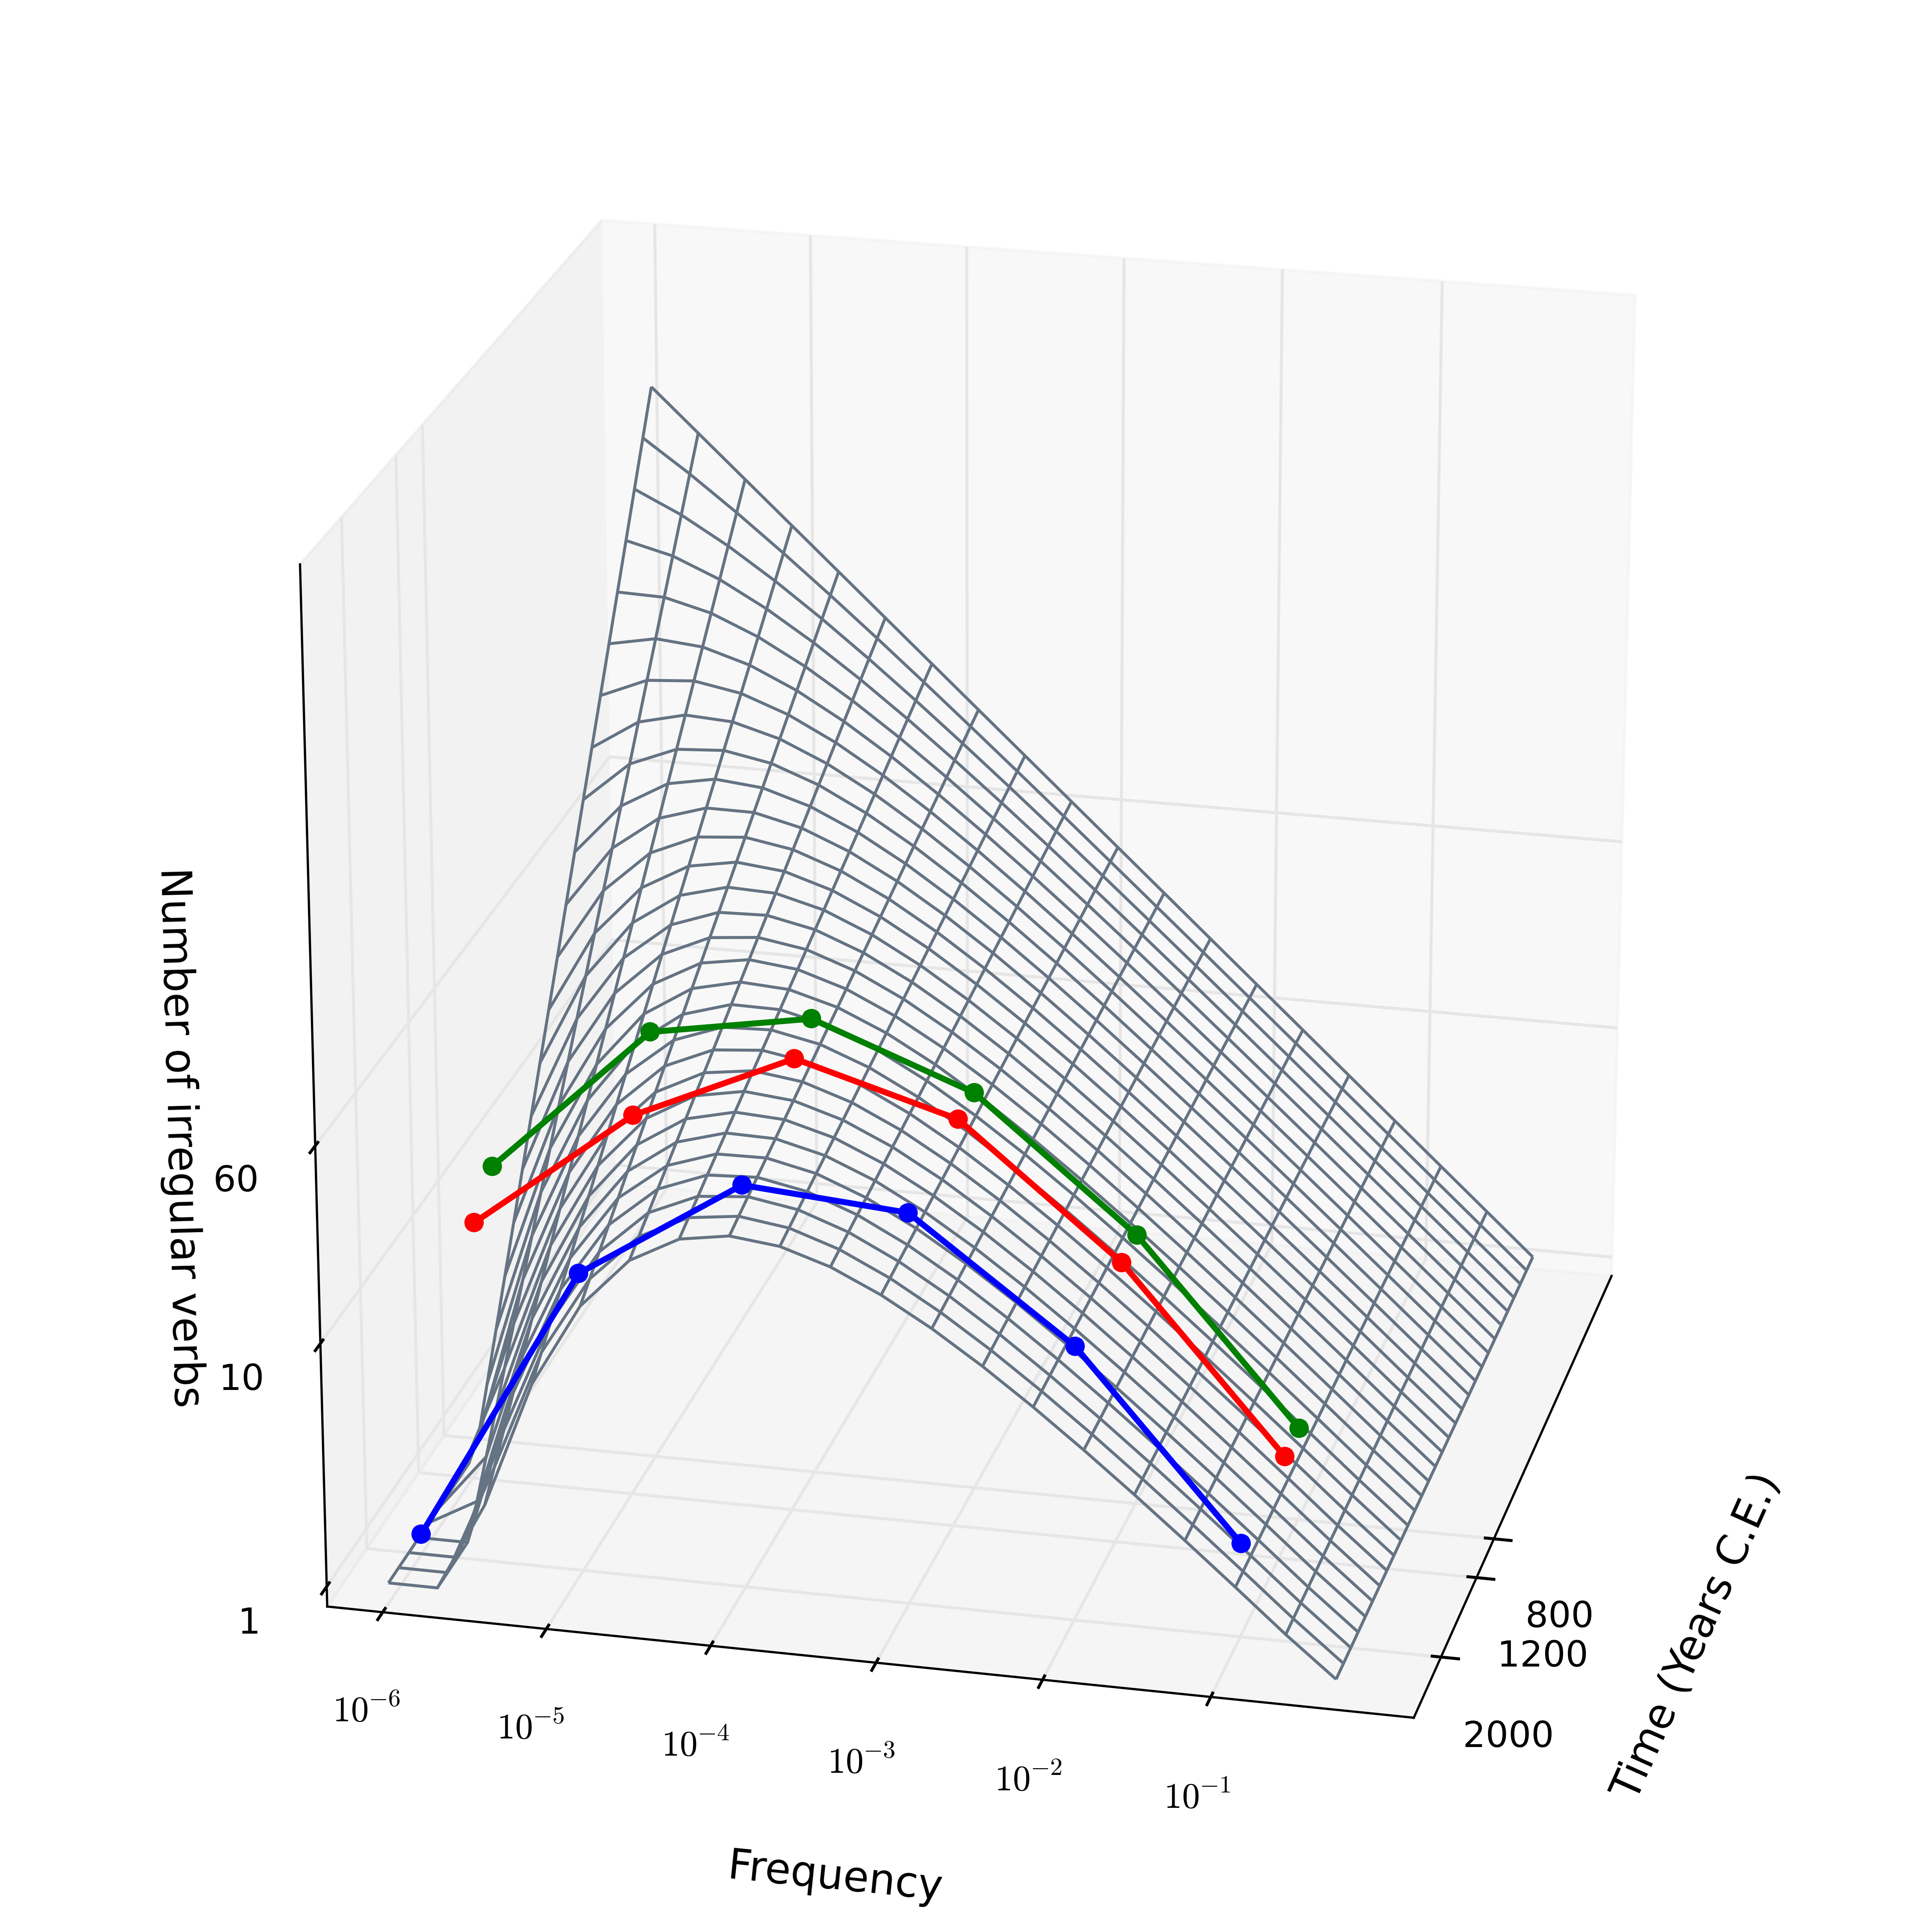
\includegraphics[width=5cm]{speed.eps}
 \caption{不規則動詞の分布\label{fig:speed}}
\end{figure}

\subsection{語形変化と外圧の影響}
Ghanbarnejadらの研究\cite{scurve}は、綴り字の改正、不規則動詞の規則化などの語形変化を
シグモイド$\sigma(x)=\frac{1}{1+\exp(-x)}$として捉え、変化を引き起こす力(外圧, 内圧)を
数値的に捉えようとしたものである.具体的には式\ref{eq:bias}の$a$を外圧、$b$を内圧(コミュニティ内のエージェントの
接触確率)とする.式\ref{eq:bias}の一般解を求め、実データに近似することで$a$、$b$の値を求める.実データは
Google Ngram Corpus\cite{google}を用いる.これは1800年から2000年に出版された電子書籍データ(3610億語)
を使ってNgram統計を行ったものである.\cite{scurve}では1-gramを用いる.

\begin{equation}
\frac{d \rho(t)}{dt}=\left(a+b\rho(t)\right)\left(1 - \rho(t)\right) \label{eq:bias}
\end{equation}

具体例としてドイツ語の綴り字の改正\cite{spelling}と、不規則動詞の規則化
について述べる.\\
 1996年にドイツ語の[\ss]を[ss]と綴るとする改正が行われた.すべての[\ss]が改正されたのではなく長母音の後ろに[\ss]
が来る場合に限りそのまま使用されている.この改正の浸透の仕方を\cite{google}を用いて年代ごとに計算する.
計算式は式\ref{eq:german}である.計算結果は、ある年代における[ss]の使用割合を示している.
そのデータを式\ref{eq:bias}に近似することで$a$、$b$の値を得る.
同様に不規則動詞も年代ごとに式\ref{eq:irre}によって、動詞ごとの規則化割合を求める.

\begin{equation}
\rho\left( t\right) = \frac{freq \left( ss \right)}{freq \left( ss \right) + freq \left( \ss \right)} \label{eq:german}
\end{equation}
\begin{equation}
\rho\left( t\right) = \frac{freq \left( regular\right)}{freq\left( regular \right) + freq\left( irregular\right) + freq\left( past participle \right) } \label{eq:irre}
\end{equation}

以上の結果を図\ref{fig:change}に示す.青のドットが実データ、オレンジの曲線が近似曲線である.
$a, b$の値からドイツ語の綴り字改正においては、大きな外圧(国規模で改正を進める)によって急激な変化
がもたらされている.逆に内部で変化を進めようとする働きは小さい.不規則動詞の規則化においては、外圧
は非常に小さく、コミュニティ内部で変化を進めようとする力が働いていると言える.

\begin{figure}[htbp]
  \begin{center}
    \begin{tabular}{c}
      \begin{minipage}{0.5\hsize}
        \begin{center}
          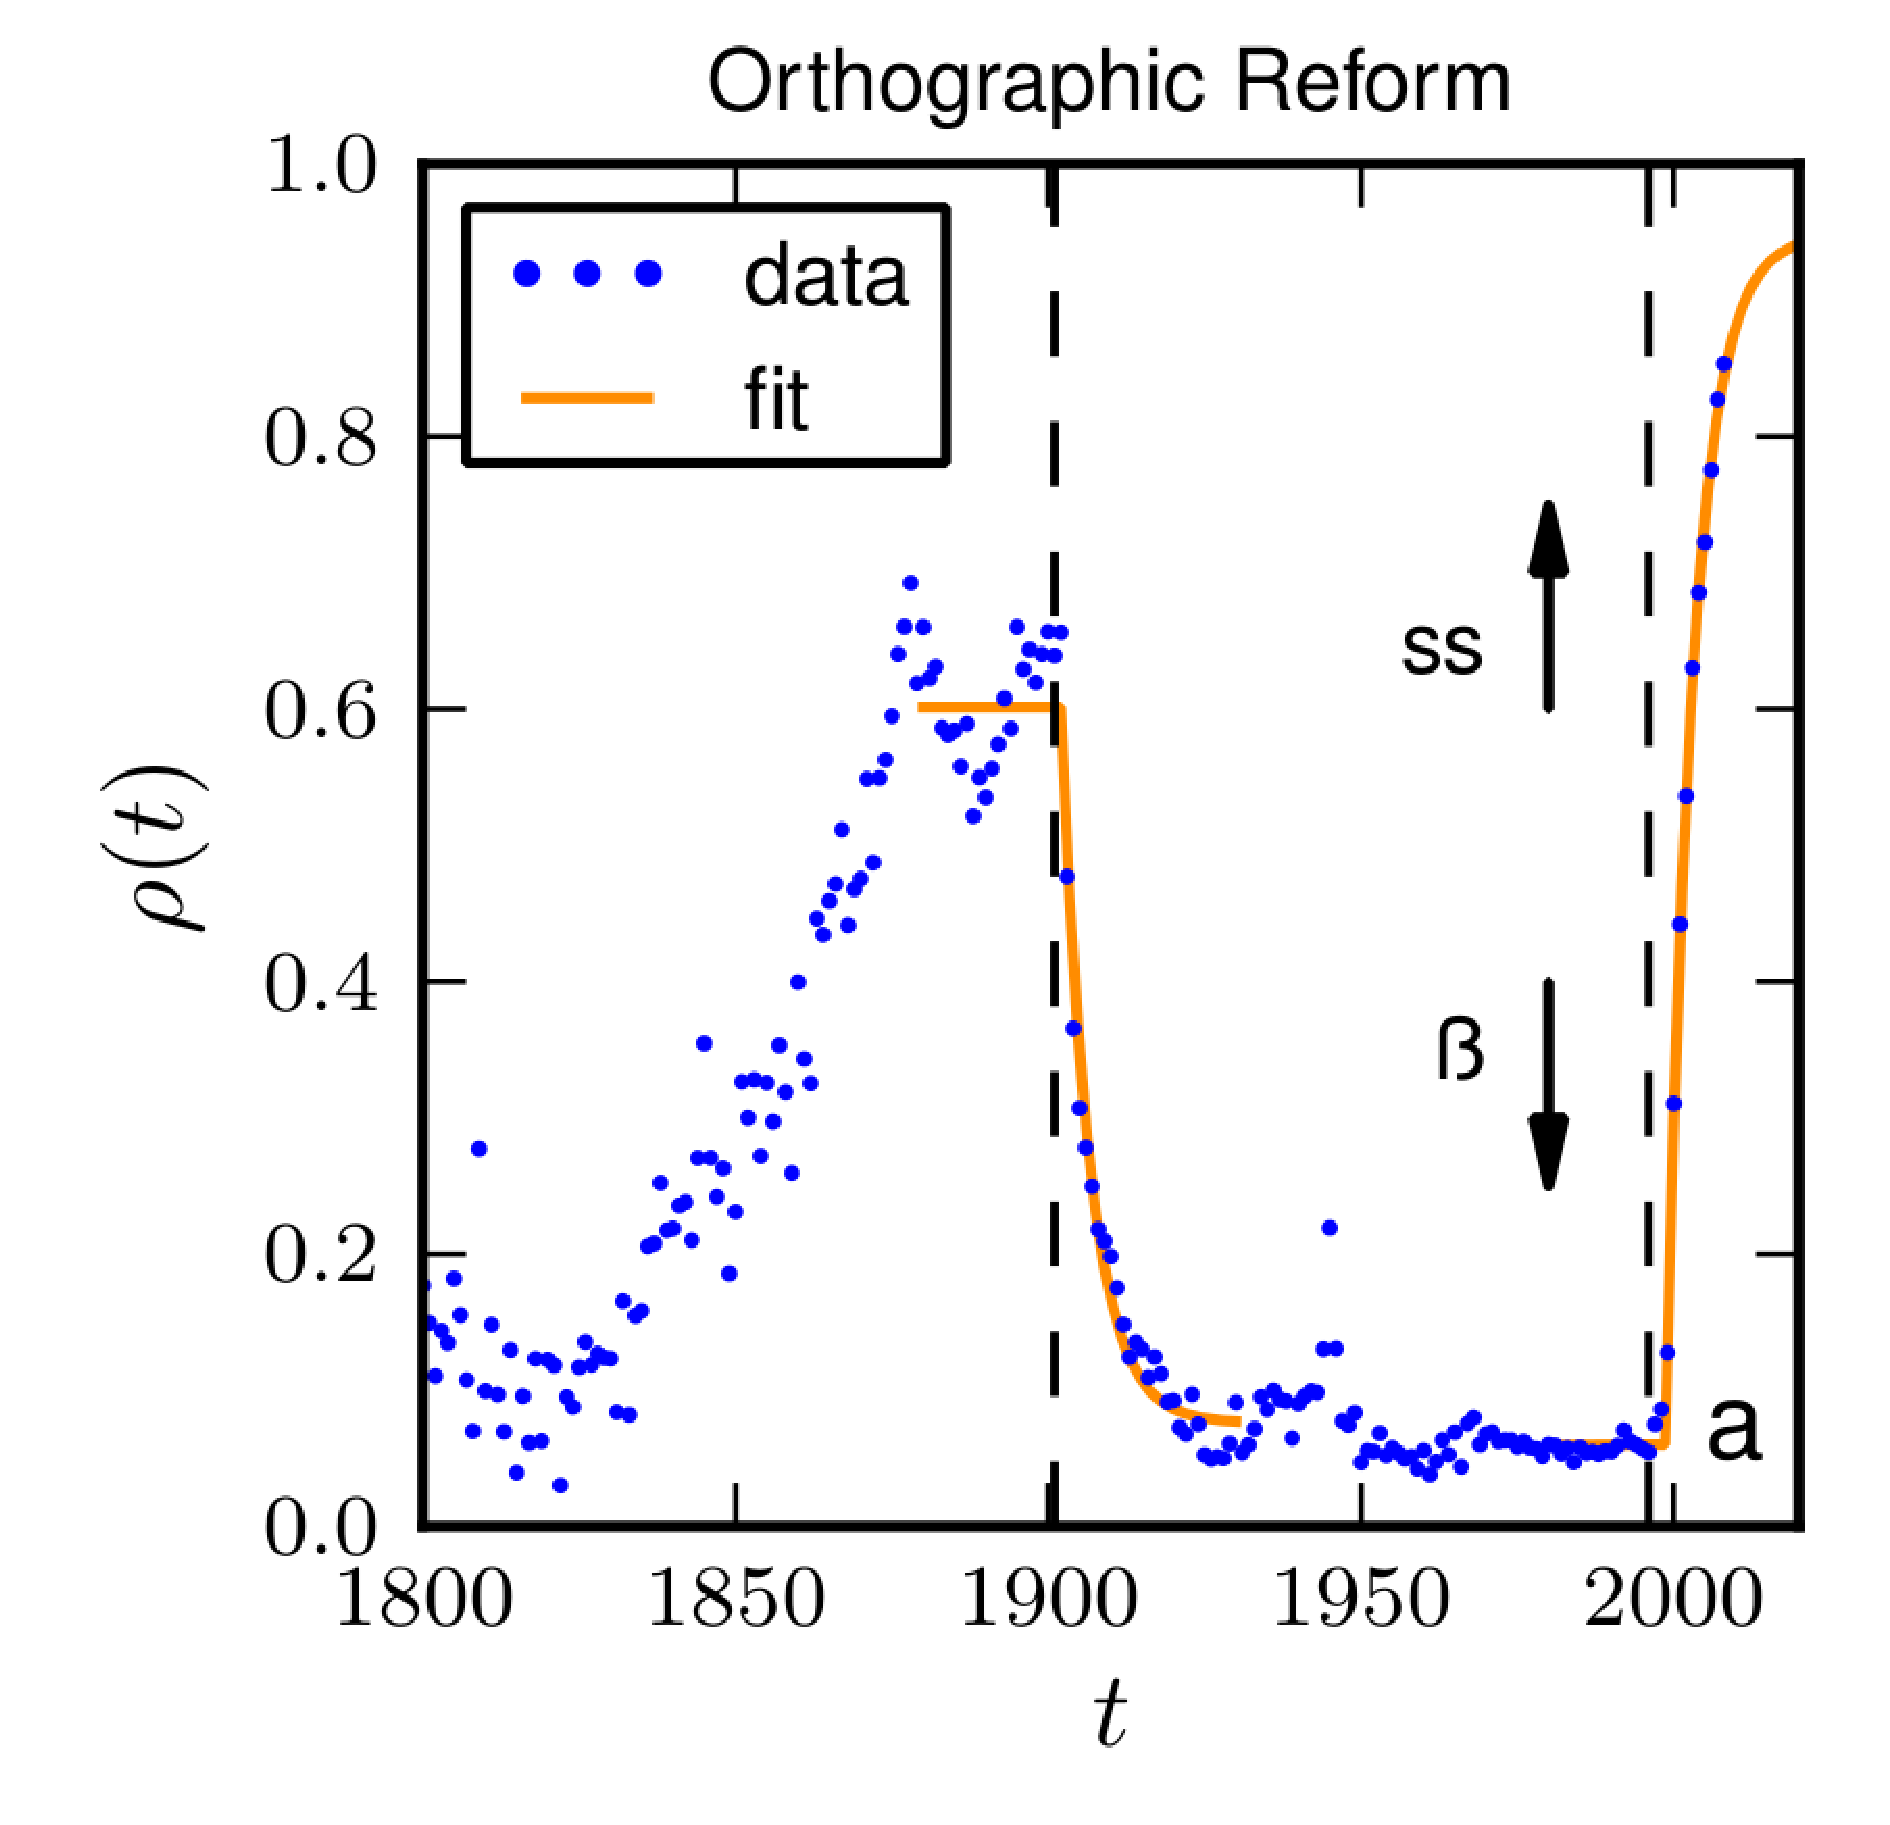
\includegraphics[clip, width=4cm]{german.eps}
          \hspace{1.0cm} \scriptsize{ドイツ語の綴り字の変化 $a=0.229, b=0.0$}
        \end{center}
      \end{minipage}

      \begin{minipage}{0.5\hsize}
        \begin{center}
          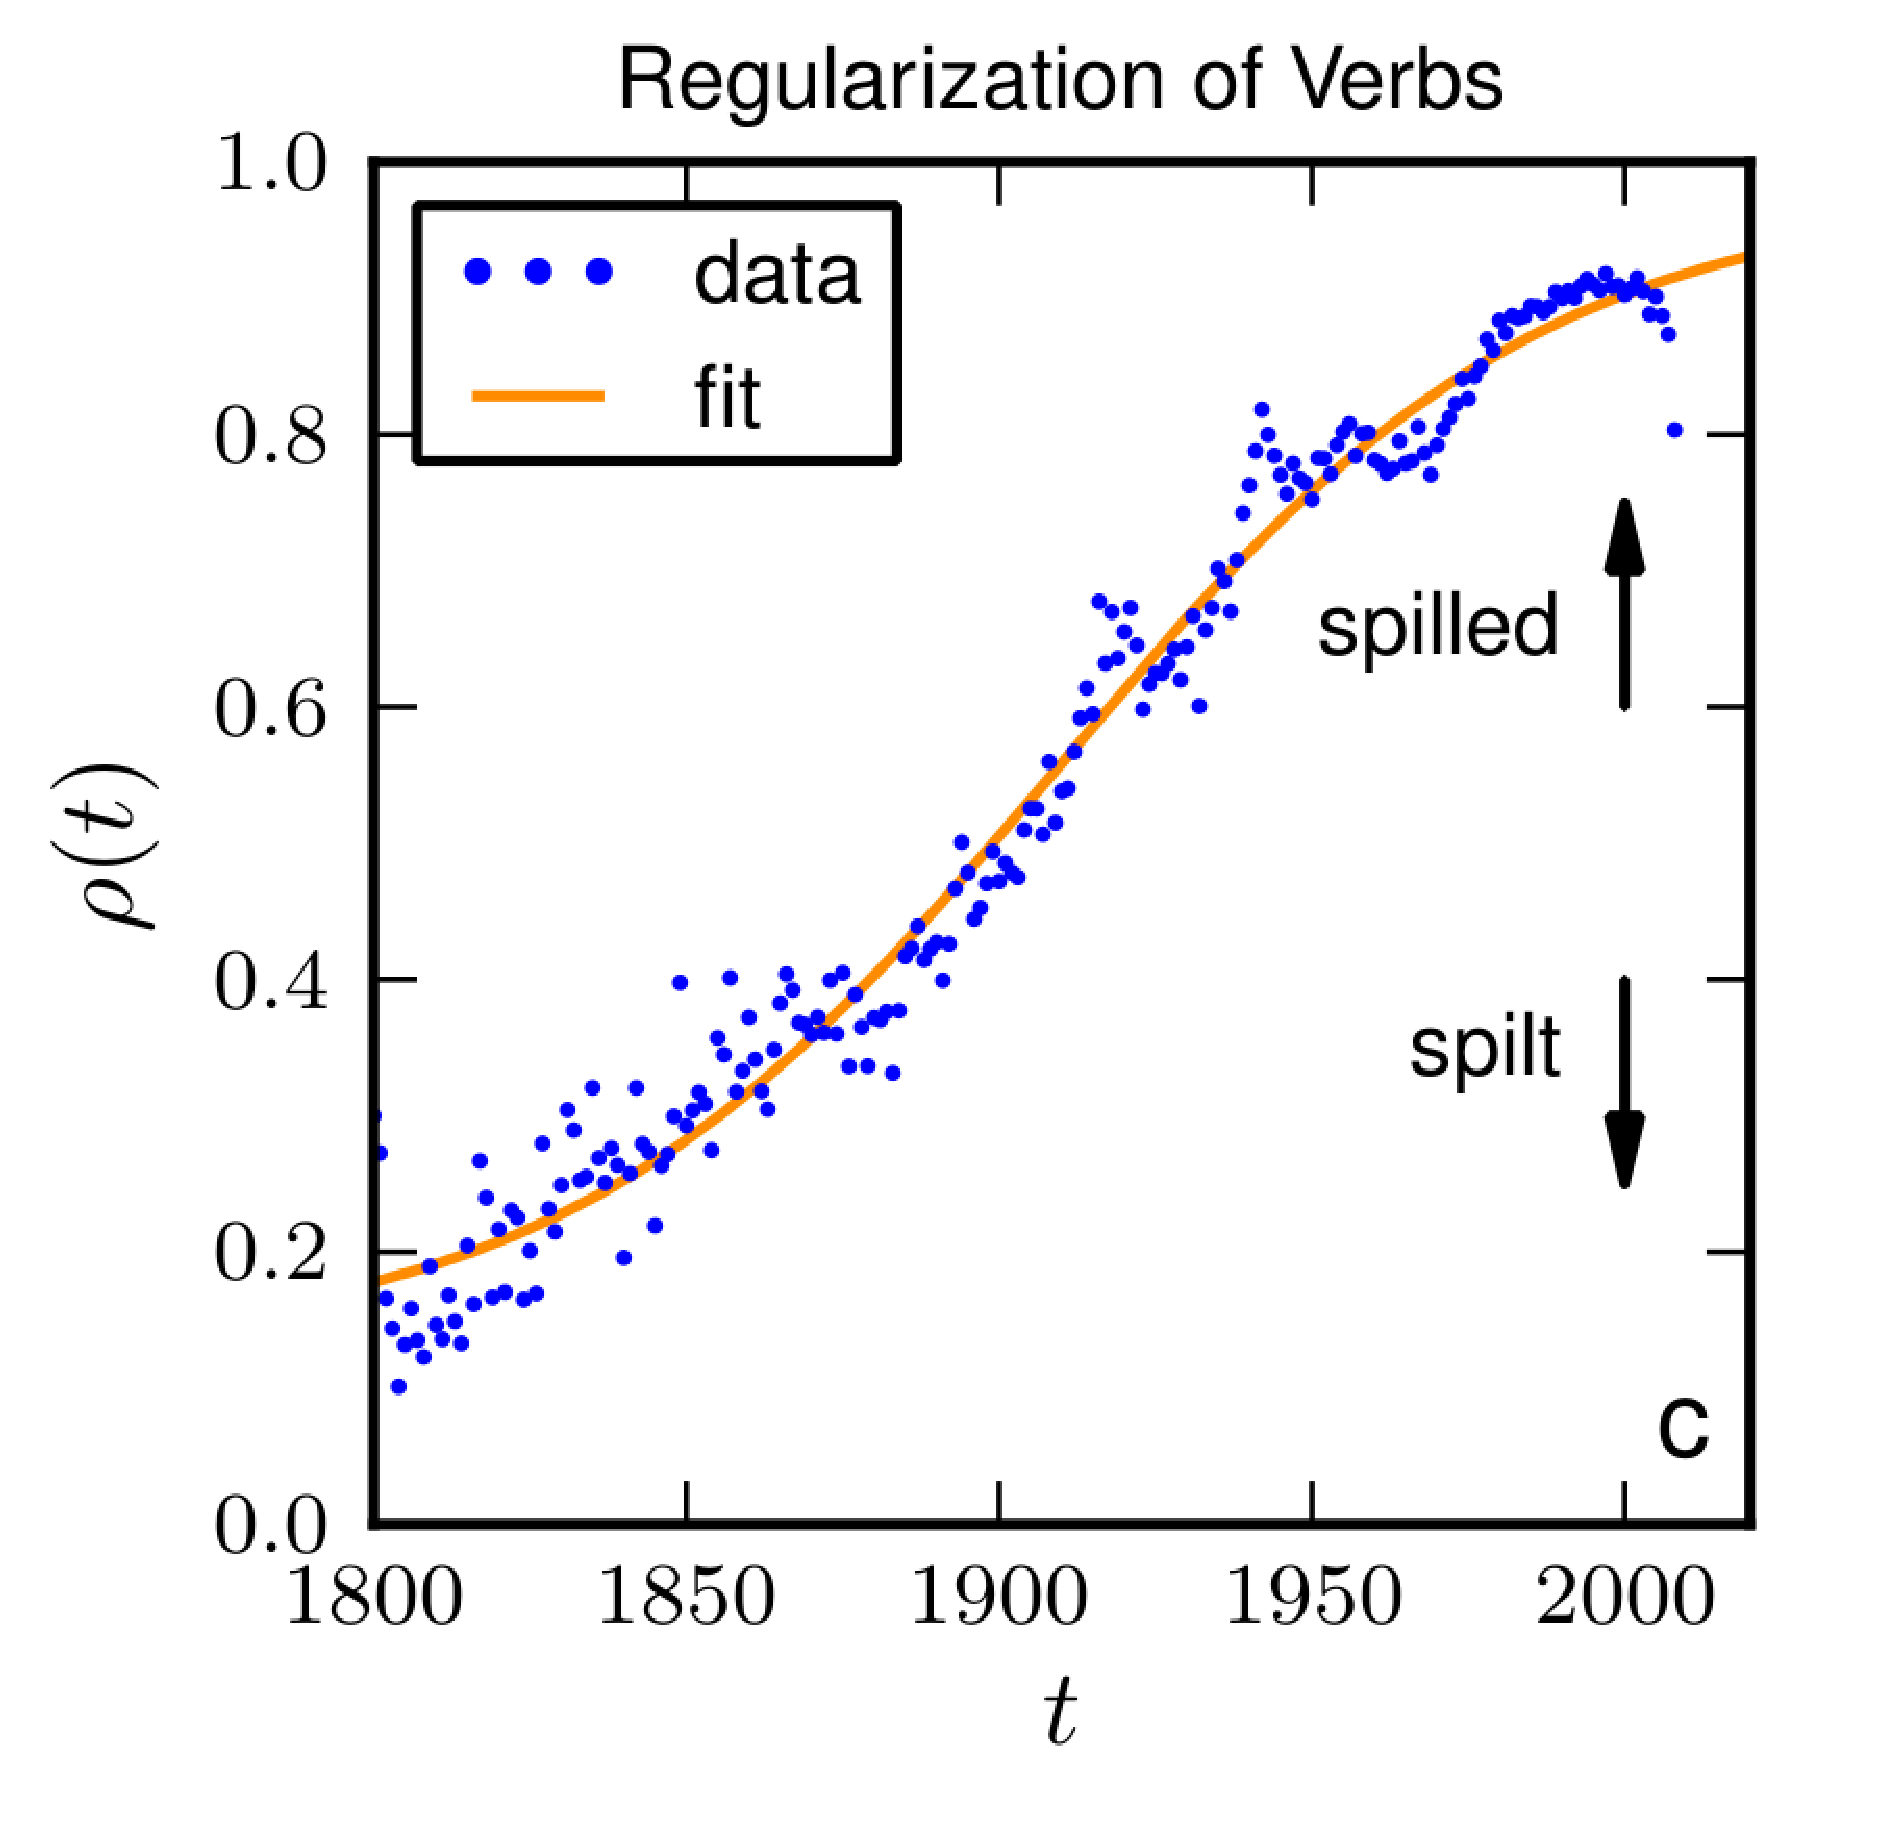
\includegraphics[clip, width=4cm]{irregular.eps}
          \hspace{1.0cm} \scriptsize{不規則動詞の規則化 \\ $a=0.001, b=0.030$}
        \end{center}
      \end{minipage}
    \end{tabular}
    \caption{\small{1800から2000年の各語形の変化\cite{scurve}より引用}} \label{fig:change}
  \end{center}
\end{figure}

\section{研究内容}
先行研究\cite{Lieberman, scurve}で、不規則動詞の規則化は頻度と時間の関数によって表現できること、
また語形変化における外圧と内圧の関係を述べた.これらは実データに基づいており、現実世界における
言語変化を表している.
よって本研究では不規則動詞の規則化は\cite{Lieberman}に従うとし、シミュレーションによって図\ref{fig:speed}
を再現する.シミュレーションの中では、人工的な言語を持ったマルチエージェント環境(コミュニティ)
を仮定する.
これは\cite{scurve}にあるようなコミュニティ内部で起こる力も表現可能にするためである.
また、外圧として人口流入を扱う.
これは言語コミュニティが様々な大きさ、頻度で外圧(人口流入)に晒されながら複数世代を通して
不規則動詞を規則化させていく状況を再現している.そして図\ref{fig:speed}を再現することによって、人口流入の
大きさ頻度も明らかにできる.
また単純に人口流入が起きれば規則化が進むのではなく、エージェント同士がコミュニケーションを行うことで
「より規則化が進むのか、またはそれを阻止しようとするのか」現実に近い状況でシミュレーションを
行うことができる.これは本研究の大きな特徴である.

\subsection{シミュレーションベースの構築}\label{sec:abst}
本研究で行うシミュレーションのベースとしてGAを用いたモデルを構築した.
表\ref{tab:ga}にGAの概要を示す.なお、実験は抽象的な設定で行い、実際には
動的に変化すると考えられる関数等もすべて固定してある.
また人口流入に関しても単純に現在は外圧とだけ考えている.

{\small
\begin{table}[htbp]
 \centering
 \caption{GAの概要\label{tab:ga}}
\small
 \begin{tabular}{l||l}
  \hline 
   個体数 & 250個体(各々が1つのコミュニティ) \\
  \hline
  PTYPE & コミュニティ内の規則化率(20\%を200と表現) \\
  \hline
  GTYPE & PTYPEの2進数(10bit) \\
  \hline
  交叉方法 & 一様交叉(60\%で交叉) \\
  \hline
  選択方法 & トーナメント方式(サイズ2) \\
  \hline
  評価関数 & ある不規則動詞の使い易さ  \\
  \hline
  突然変異 & 外圧と仮定 \\
  \hline
  バイアス & 正規分布(変化を加速させる働き)\\
  \hline
\end{tabular}
\end{table}
}

表\ref{tab:ga}における評価関数、突然変異、バイアスについて以下で説明を行う.
\subsection{評価関数}\label{sec:evalfunc}
ある不規則動詞について、それが不規則変化、規則変化どちらが使い易い
のか(適応度)を評価する関数である.この関数は環境によって動的に変化することが予想される.
関数の形を決める要因は、使用頻度やエージェント同士の会話の伝わりやすさなどが
考えられる.
\subsection{突然変異とバイアス}\label{sec:mutatebias}
本研究では突然変異は、コミュニティにかかる外圧と考えている.つまり、外圧がかかれば
変化が加速されるバイアスがかかる.例えばコミュニティ内において外圧によって規則化が進んでいるとする.
コミュニティ全体が不規則変化、規則変化を使用する人間が混在する不安定な状況化にとどまることは考えにくい.
よって、抑える力が働かない限り規則化は推し進められる.この力をバイアスとして表現する.また、外圧の影響
が徐々に浸透していき、浸透しきれば影響は少なくなると言い換えることもできる.バイアスは図\ref{fig:bias}
の正規分布で与えられる.モデル上では外圧がかかった世代から何世代かに渡り、各個体のPTYPEを変化の
方向に押し上げる働きをする.上記の例に従えば各個体に値を加算し規則化率を押し上げていく.
加算する値は正規分布に従い、小さい値から徐々に大きな値になりまた小さくなっていく.

\begin{figure}[htbp]
 \centering
 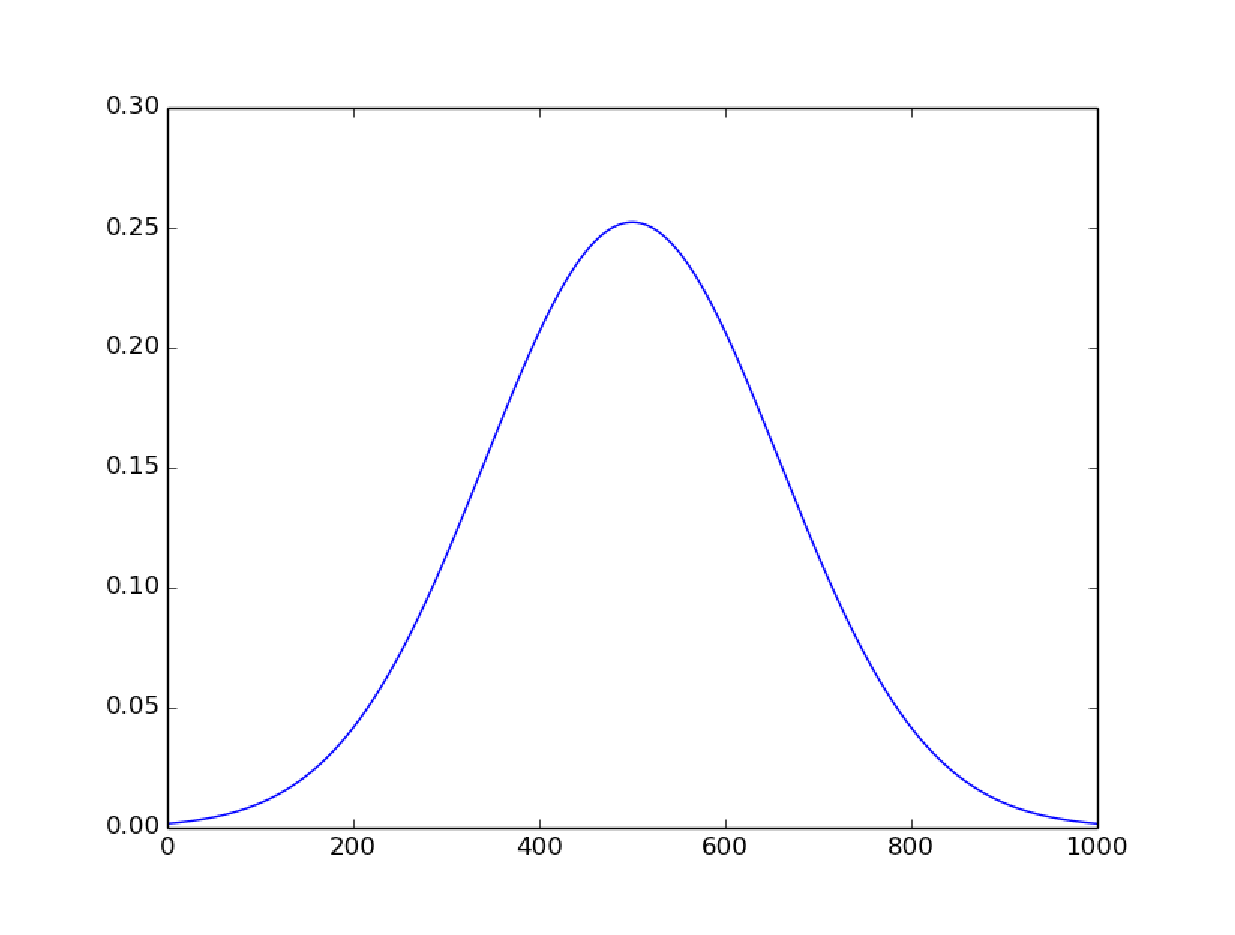
\includegraphics[width=5cm]{bias.eps}
 \caption{変化を加速させるバイアス\label{fig:bias}}
\end{figure}

\subsection{実験}
\ref{sec:evalfunc}、\ref{sec:mutatebias}の元、規則化が進行するシミュレーションを行った.
GAの設定は表\ref{tab:ga}と同様である.コミュニティの規則化率はスタート時20\%とし、評価関数
は分散30000、平均1000の正規分布を仮定した(固定).つまり規則化を進めたほうが適応度が上がる設定である.
外圧がかかる世代は50世代目とし、その後20世代にわたってバイアスがかかるよう設定した.図\ref{fig:result}に100回
シミュレーションを行った平均を示す.
\begin{figure}[htbp]
 \centering
 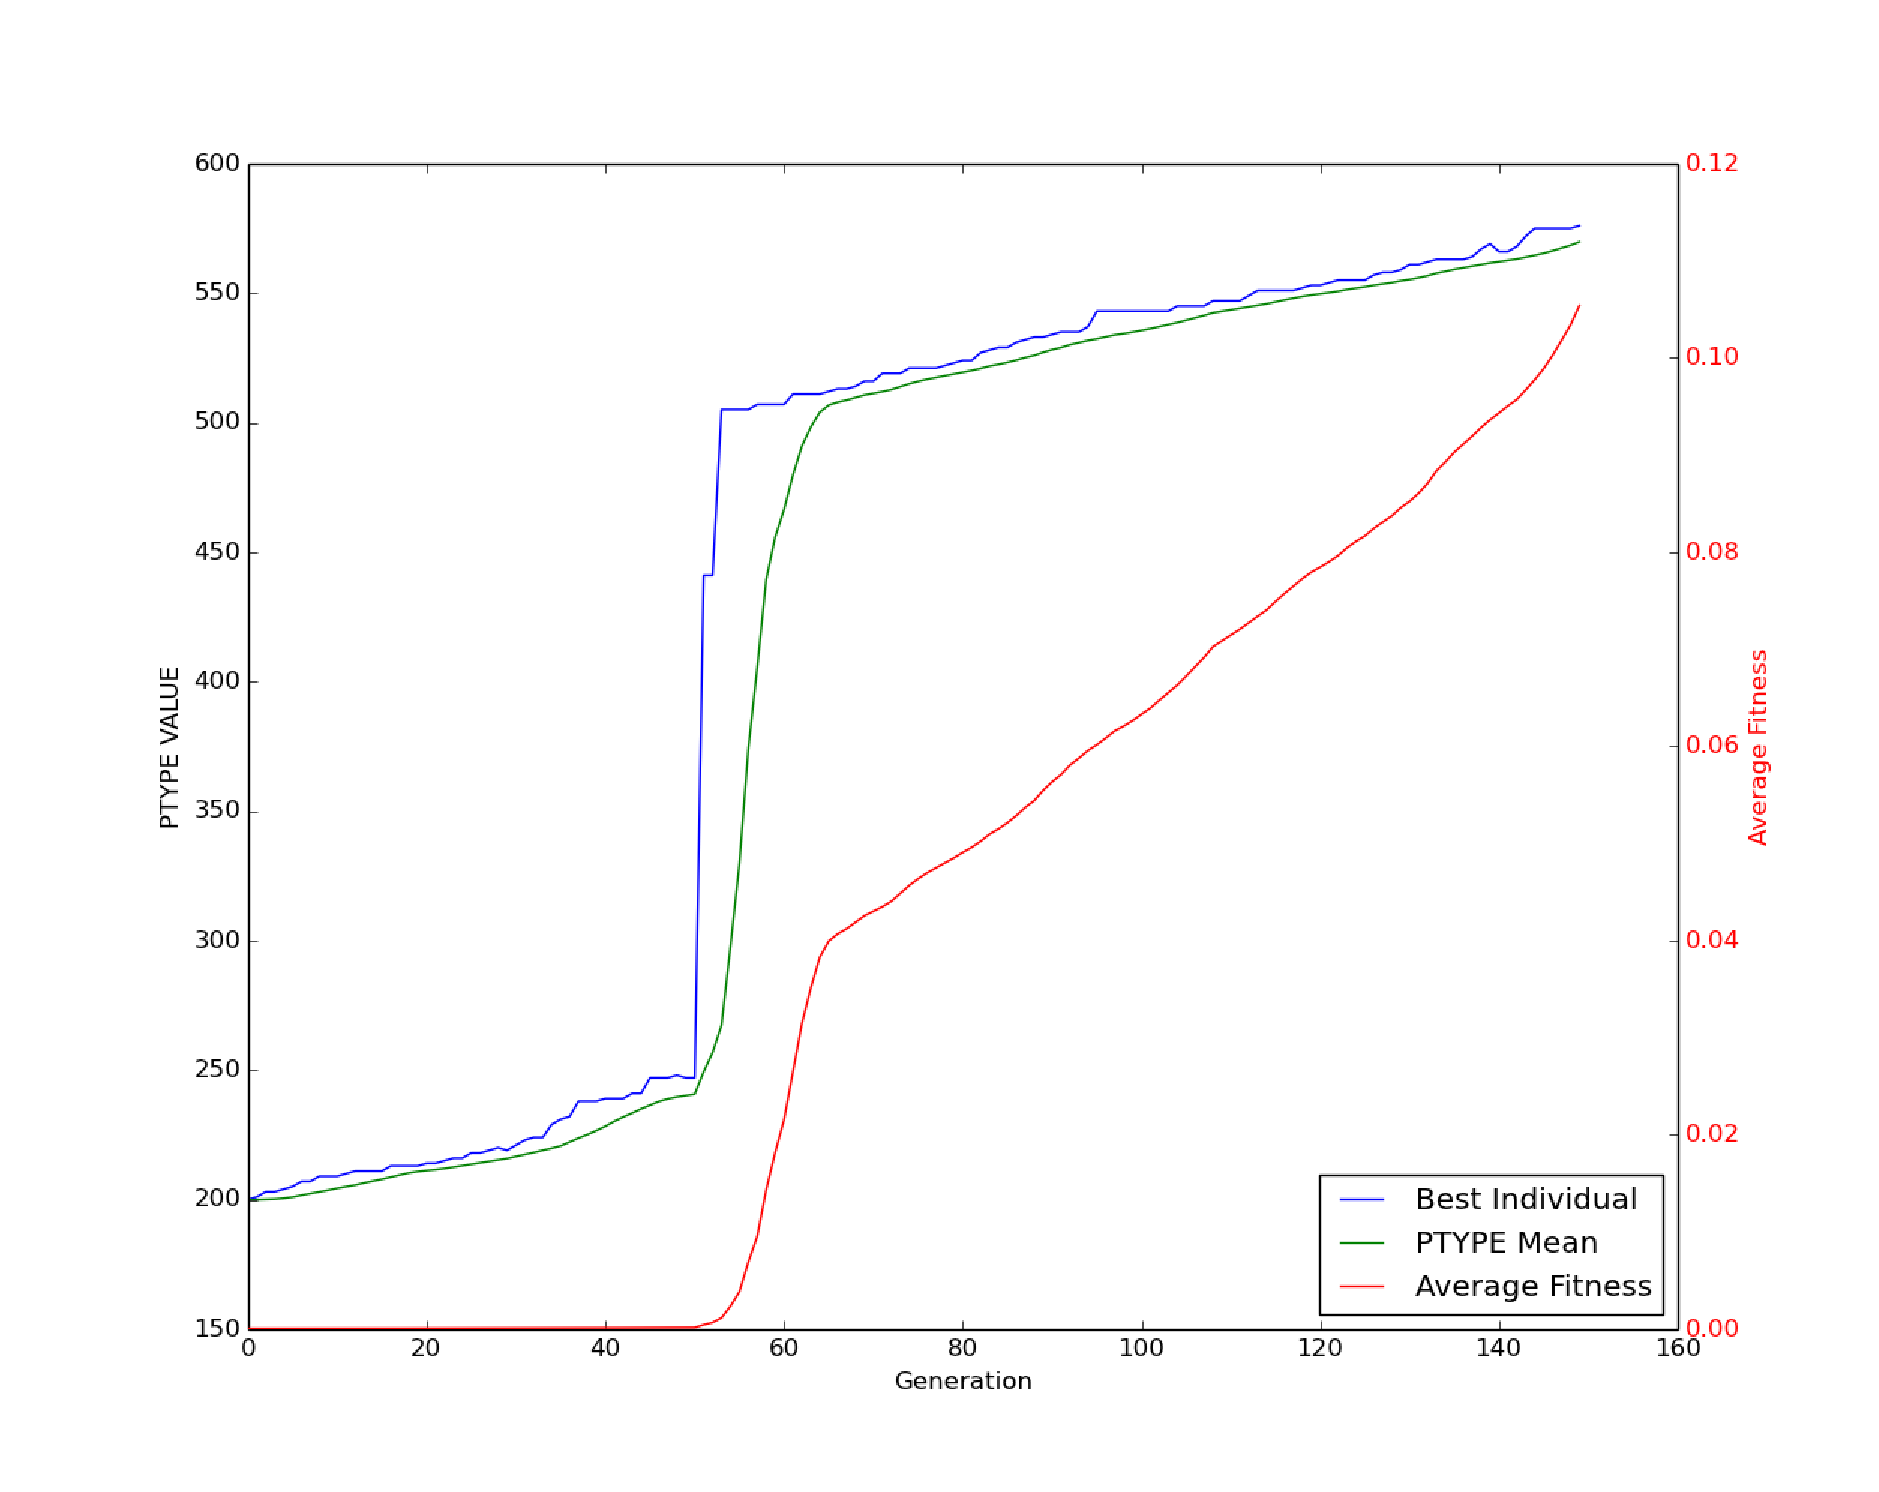
\includegraphics[width=5cm]{result.eps}
 \caption{変化を加速させるバイアス\label{fig:result}}
\end{figure}

図\ref{fig:result}の縦軸は全コミュニティの平均規則化率を示す.図中の緑の曲線がその移り変わりを表現している.
青線は最も適応度の高いコミュニティの規則化率、赤線は平均適応度である.
緑の曲線からバイアスがかかりはじめた50世代目から徐々に上昇を始め、最も強いバイアスがかかる中間付近では
急激な上昇を見せている.その後はまたゆっくりとした変化に収束する様子が表現できている.

\section{まとめと今後の課題}
GAを元にシミュレーションモデルの作成を行った.外圧が加われば変化が加速されるという実際の語形変化に
則した変化を意図的な突然変異と数世代に渡るバイアスという形で表現した.今後の課題は、規則化だけでなく
不規則化に対応できようなモデルに拡張する必要がある.特にバイアスを動的に設定できる仕組みを導入する.
例えば外圧の大きさだけ設定すれば、バイアスの大きさや影響する世代を自動的に判断し実行する.\\
 またコミュニティの設定のために、人工的な動詞の作成やエージェントコミュニケーションを導入し
コミュニティの状況によって変化する評価関数(複数の要因パラメータを持ち、関数の形
が変化する)を作成する.現段階では外圧をただPTYPEの値を変化させるだけで扱っている.今後は人口流入
を明確に定義し、扱えるようにする.

{\scriptsize
\begin{thebibliography}{9}
\addcontentsline{toc}{section}{\refname}% 目次に追加
 \bibitem{pinker}
   \emph{Pinker, S. The irregular verbs. Landfall 83–85 (Autumn issue, 2000)}
 \bibitem{pinker2}
   \emph{Pinker, S , Prince, A. On language and connectionism: analysis of a parallel distributed processing model of language acquisition. Cognition 28,p73-193 (1988)}
 \bibitem{iba_ga}
   \emph{伊庭 斉志, 遺伝的アルゴリズムの基礎-GAの謎を解く オーム社(1994)}
 \bibitem{english_div}
   \emph{Tom McArthur, THE ENGLISH LANGUAGES, Cambridge University Press (1998), 英語系諸言語, 牧野武彦 監修, 山田 茂, 中本 恭平 訳, 三省堂 (2009)}
 \bibitem{philip}
   \emph{Philip Gooden, THE STORY OF ENGLISH (2009), 物語 英語の歴史, 田口孝夫 監修, 悠書館 (2012)}
  \bibitem{Lieberman}
    \emph{Erez Lieberman, Jean-Baptiste Michel, Joe Jackson, Tina Tang , Martin A. Nowak, Quantifying the evolutionary dynamics of language. Nature Vol449 (11 October 2007)}
  \bibitem{celex}
    \emph{CELEX http://wwwlands2.let.kun.nl/members/software/celex.html}
  \bibitem{scurve}
    \emph{Ghanbarnejad, Fakhteh, et al. Extracting information from S-curves of language change. Cornell University Library arXiv preprint arXiv:1406.4498 (2014)}
  \bibitem{spelling}
    \emph{Chris Upward, Spelling Reform in German. Journal of the Simplified Spelling Society, J21, 1997-1 pp22-24,36}
  \bibitem{google}
    \emph{Google Ngram Viewer, https://books.google.com/ngrams}
\end{thebibliography}
}
\end{document}
